\newpage
\FloatBarrier
\section{An alternating Wall} \label{alternatingWall}
\begin{table}[h!]
	\begin{tabular}{c c}
	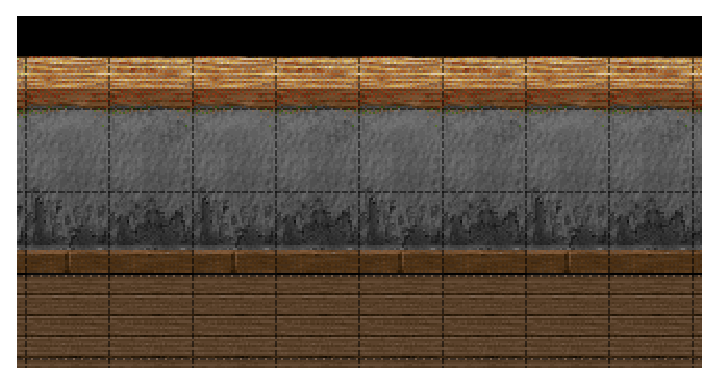
\includegraphics[scale=0.5]{Example/LoneCoder/alternatingwalls/desired.eps} &
	\includegraphics[scale=0.5]{Example/LoneCoder/alternatingwalls/setlayer.eps} \\
	\end{tabular}
  \caption{The left picture shows the desired wall. Vertically the tiles are alternating (Every second tile of the base board has a notch). The right picture shows the set layer.}
  \label{desiredAlternativeWall}
\end{table}

\begin{wrapfigure}{r}{0.45\textwidth}
   \begin{tabular}{|c|l|}
   \hline
   tile layer & name \\
   \hline
   \hline
	\includegraphics[scale=0.5]{Example/LoneCoder/alternatingwalls/regions.eps} & Regions \\
	\hline
	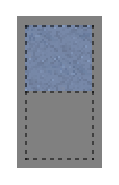
\includegraphics[scale=0.5]{Example/LoneCoder/alternatingwalls/input.eps} & Input\_set\\
	\hline
	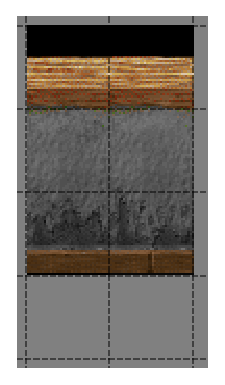
\includegraphics[scale=0.5]{Example/LoneCoder/alternatingwalls/output.eps} & Output\_Walls\\
	\hline
	\end{tabular}
  \caption{The region tile layer(top), the input tile layer(mid) and the output tile layer(bottom)}
  \label{alternatingWallsRule}
\end{wrapfigure}

This example will demonstrate how a wall as a transition between a walkable 
area and the nonwalkable black void can easily be setup. 
As input a dedicated set layer will be used.

The structure of the input, output and region layer is very similar to the example~\ref{basic_shoreline}.
The main difference is the different size. Since the wall contains multiple tiles in height,
the height of the rulelayers is different as well. Vertically the tiles are also alternating. 
As you can see in figure~\ref{desiredAlternativeWall}, every second tile displaying the base board of the Wall has a notch for example.

Hence the region in which this Automapping rule should be defined is of 4 tiles in height and 
2 tile in width. Therefore we need a layer called \emph{Regions} and it will have 8 tiles placed
to indicate this region. In figure~\ref{alternatingWallsRule} the top graphics shows such a region
layer.

The input layer has the following meaning: \emph{If there are 2 vertical adjacent brown tiles in the set layer
and in the 3x2 tiles above there are no brown tiles, this rule matches.}
Only the lowest 2 coordinates contain the brown tile. The upper coordinates contains no tile. 
(It is not an invisible tile, just no tile at all.)
The input layer called \emph{Input\_set} is depicted in the middle of 
figure~\ref{alternatingWallsRule}. 

The output consists of only one layer as well called \emph{Output\_Walls}.
It contains the actual wall tiles.

When trying to match the input layer to the desired set layer (right picture of figure~\ref{desiredAlternativeWall},
you will see it matches all way long, no matter of the vertical adjustment.

Hence when we use the rule as discussed now, we will get not the desired result, but this rule
overlaps itself. The overlapping problem is shown in figure~\ref{problemAlternativeWall}

\begin{table}
	\begin{tabular}{c c}
	\includegraphics[scale=0.5]{Example/LoneCoder/alternatingwalls/firstattempt.eps} &
	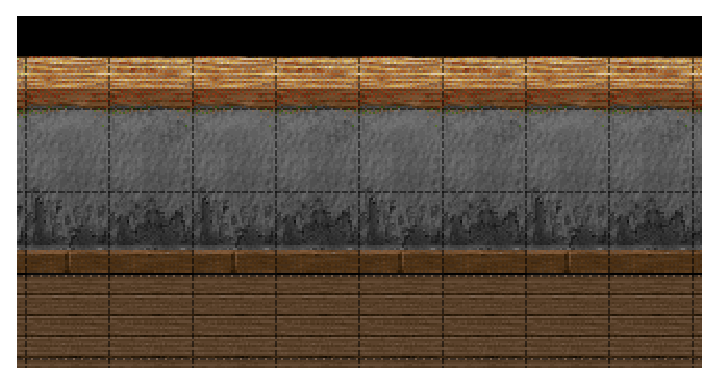
\includegraphics[scale=0.5]{Example/LoneCoder/alternatingwalls/desired.eps} \\
	\end{tabular}
  \caption{The left picture shows the first attempt of the wall. Only the first parts of the wall is created, 
  the second parts have been overwritten by another instance of this rule.
  The right picture shows the correct version by setting the map property \emph{NoOverlappingRules} to true.}
  \label{problemAlternativeWall}
\end{table}

Since the overlapping is not desired, we can turn it off by adding a map property to the rulemap
\emph{NoOverlappingRules} and setting it to "true".

Mind, that the map property applies for all rules on that rule map.



